\documentclass[12pt,a4paper,dvipdfmx]{jarticle}
%
\topmargin=-5mm
\oddsidemargin=-5mm
\evensidemargin=-5mm
\textheight=235mm
\textwidth=165mm
%
\title{FDPS講習会の手引}
\author{谷川衝、岩澤全規、細野七月、似鳥啓吾、村主崇行、牧野淳一郎}
\date{\today}
%\pagestyle{empty}
\usepackage[dvipdfmx]{graphicx}
\usepackage{wrapfig}
\usepackage{lscape}
\usepackage{amssymb}
\usepackage{amsmath}
\usepackage{bm}
\usepackage{setspace}
%\usepackage{listings,jlisting}
\usepackage{color}
\usepackage{ascmac}
\usepackage{here}
\usepackage[dvipdfmx]{hyperref}
\usepackage{pxjahyper}

\newcommand{\underbold}[1]{\underline{\bf #1}}
\newcommand{\redtext}[1]{\textcolor{red}{#1}}

%\setcounter{secnumdepth}{4}
%%%%%%%%%%%%%%%%%%%%%%%%%%%%%%%%%%
\setcounter{secnumdepth}{5}
\makeatletter
\newcommand{\subsubsubsection}{\@startsection{paragraph}{4}{\z@}%
{1.5\baselineskip \@plus.5\dp0 \@minus.2\dp0}%
{.5\baselineskip \@plus2.3\dp0}%
{\reset@font\normalsize\bfseries}
}
\newcommand{\subsubsubsubsection}{\@startsection{subparagraph}{5}{\z@}%
{1.5\baselineskip \@plus.5\dp0 \@minus.2\dp0}%
{.5\baselineskip \@plus2.3\dp0}%
{\reset@font\normalsize\itshape}
}
\makeatother
\setcounter{tocdepth}{5}
%%%%%%%%%%%%%%%%%%%%%%%%%%%%%%%%%%

\begin{document}
\maketitle
\tableofcontents

\newpage

\section{プログラム}

\begin{itemize}

\item 13:00 -- 14:00 FDPSの講義
  \begin{itemize}
  \item イントロダクション (牧野淳一郎)
  \item 概要説明 (谷川衝)
  \item FDPS詳細1 -- APIと内部構造 (岩澤全規)
  \item FDPS詳細2 -- サンプルコード解説 (細野七月)
  \item Q\&A
  \end{itemize}

\item 14:00 -- 15:30 FDPSの実習
  \begin{itemize}
  \item FDPSのインストール
  \item サンプルコードの使用1 (重力N体シミュレーションコード)
  \item サンプルコードの使用2 (SPHシミュレーションコード)
  \end{itemize}

\item 15:30 -- 17:00 FDPS使用に関する相談

\end{itemize}

\newpage

\section{概要}
今回はこんな事をしてFDPSを使ってもらいます


\section{FDPSの実習}

\subsection{準備}

\subsubsection{FOCUSの計算機を用いる場合}
まずは、FOCUSの計算機にログインするまでの手順を紹介する。講習用PCの電源
をつけたら、デスクトップ左下のスタートメニューボタンを押し、ウィンドウ
ズメニューを開く。正しく開けたら図\ref{fig:startmenu}のようになるはずで
ある。
\begin{figure}
  \begin{center}
    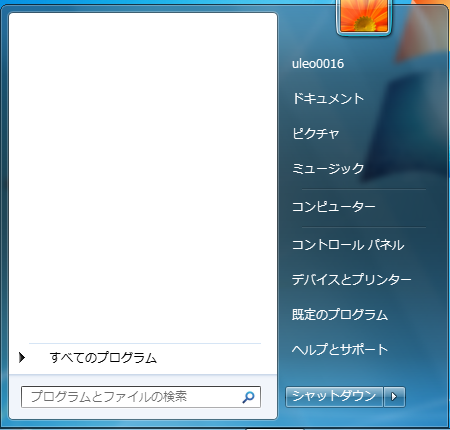
\includegraphics[clip, width=10.0cm]{fig/startmenu_.png}
  \end{center}
  \caption{}
  \label{fig:startmenu}
\end{figure}

次に、Cygwin-Xというフォルダを開き、XWin Serverを起動する(図\ref{fig:cygwinX2}参照)。
起動に成功したら、XWin Serverが図\ref{fig:xboot}の様に起動するはずである。
\begin{figure}
  \begin{center}
    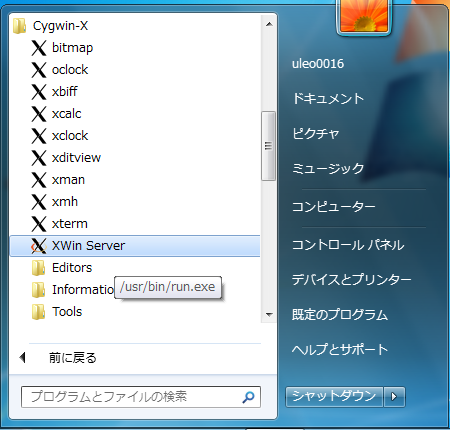
\includegraphics[clip, width=10.0cm]{fig/cygwin-X2_.png}
  \end{center}
  \caption{}
  \label{fig:cygwinX2}
\end{figure}

\begin{figure}
  \begin{center}
    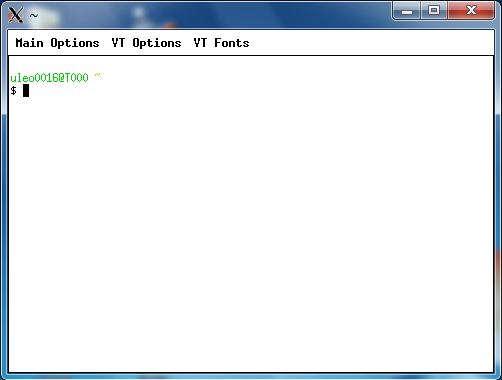
\includegraphics[clip, width=10.0cm]{fig/xboot_.png}
  \end{center}
  \caption{}
  \label{fig:xboot}
\end{figure}

次に、計算用ノードにログインを行う。
今回の実習ではPuTTYというソフトウェアを使う。
スタートメニューから、PuTTYというフォルダをクリックする(図\ref{fig:PuTTY})。
フォルダが開くはずなのでPuTTYをクリックし、起動する(図\ref{fig:PuTTY2})。
\begin{figure}
  \begin{center}
    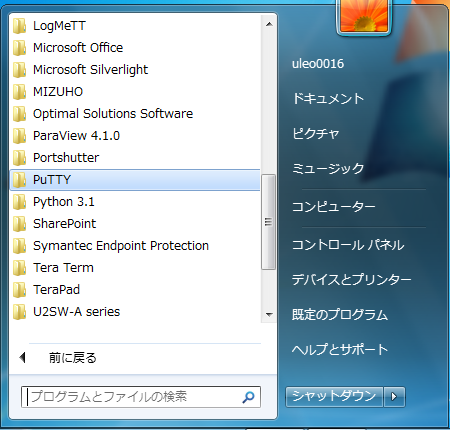
\includegraphics[clip, width=10.0cm]{fig/PuTTY_.png}
  \end{center}
  \caption{}
  \label{fig:PuTTY}
\end{figure}

\begin{figure}
  \begin{center}
    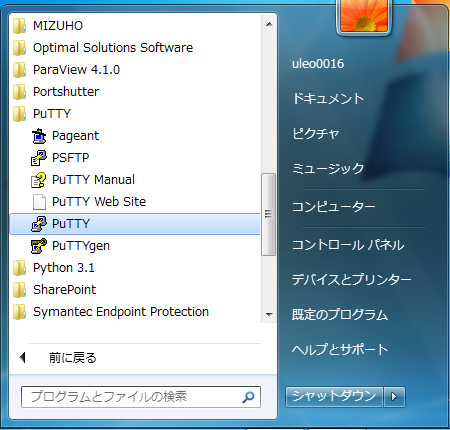
\includegraphics[clip, width=10.0cm]{fig/PuTTY2_.png}
  \end{center}
  \caption{}
  \label{fig:PuTTY2}
\end{figure}
PuTTYが起動すると、図\ref{fig:PuTTY3}の様なメニューが開かれるはずである。
この、``HostName (or IP address)''と書いてあるボックスに、
「ff01.j-focus.jp」または「ff02.j-focus.jp」の好きな方を書く(図\ref{fig:PuTTY4})。
次に、左側のメニューのSSHの左側の+をクリックし、X11を選択する。
そこにある``Enable X11 forwarding''の左のチェックボックスをオンにする(図\ref{fig:PuTTY5})。
これらが終わったら、Openボタンを押す。
\begin{figure}
  \begin{center}
    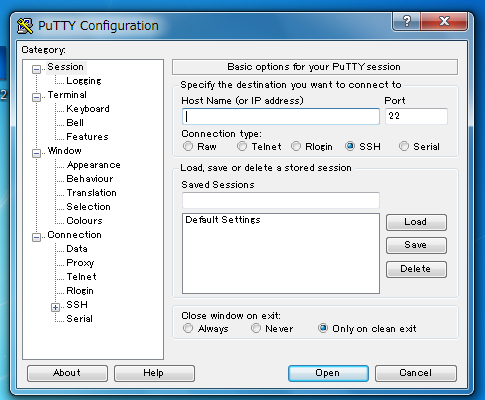
\includegraphics[clip, width=10.0cm]{fig/PuTTY3_.png}
  \end{center}
  \caption{}
  \label{fig:PuTTY3}
\end{figure}

\begin{figure}
  \begin{center}
    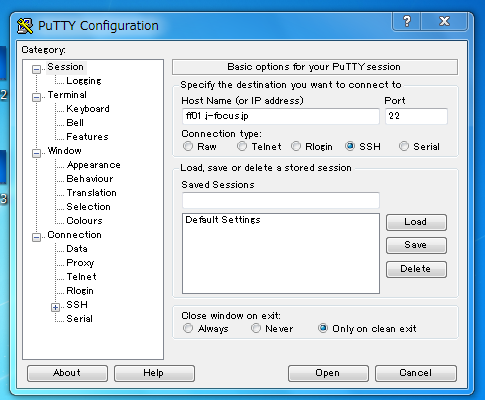
\includegraphics[clip, width=10.0cm]{fig/PuTTY4_.png}
  \end{center}
  \caption{}
  \label{fig:PuTTY4}
\end{figure}

\begin{figure}
  \begin{center}
    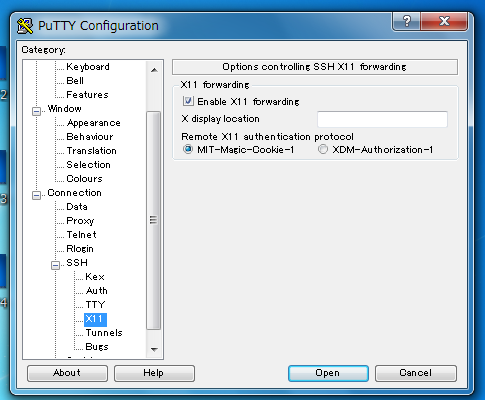
\includegraphics[clip, width=10.0cm]{fig/PuTTY5_.png}
  \end{center}
  \caption{}
  \label{fig:PuTTY5}
\end{figure}

Openを押すとログイン画面が開かれる(図\ref{fig:login2})。
ユーザー名とパスワードを入力すればログインは完了である。
\begin{figure}
  \begin{center}
    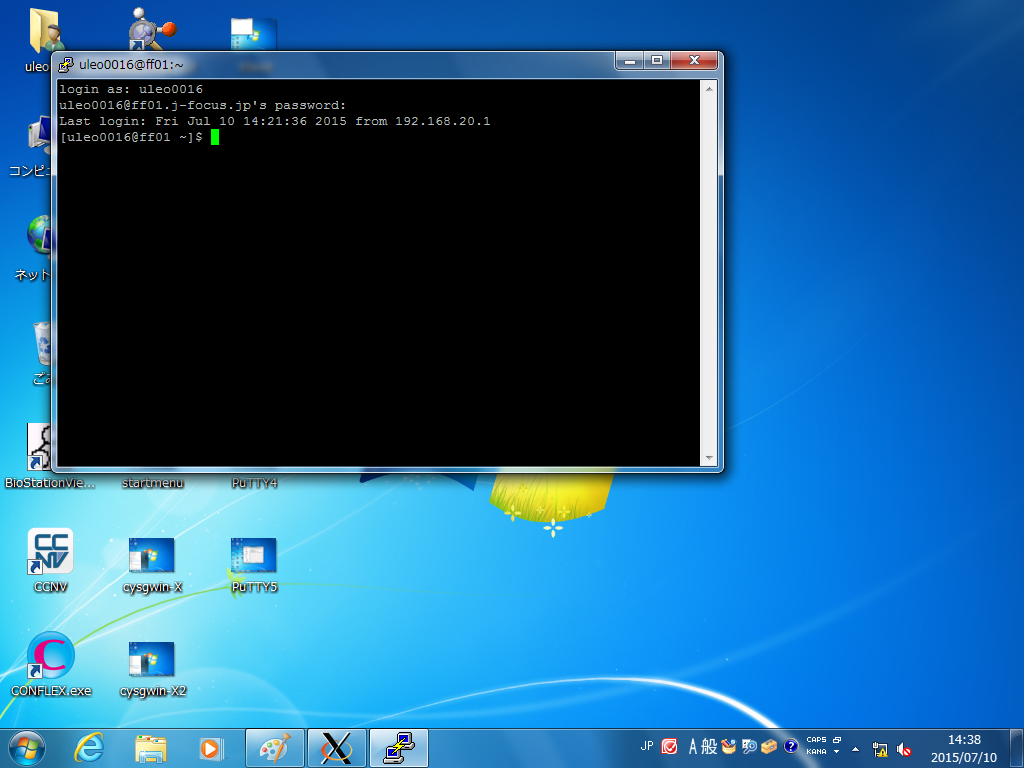
\includegraphics[clip, width=10.0cm]{fig/login2.png}
  \end{center}
  \caption{}
  \label{fig:login2}
\end{figure}

FOCUSの計算機にログインしたら、以下のコマンドを実行する。
\begin{screen}
\begin{verbatim}
$ module load gnu/openmpi165
\end{verbatim}
\end{screen}

以下のコマンドを実行し、FDPSを自分のカレントディレクトリにコピーする
(「\verb|$|」はコマンドプロンプトであるので、「\verb|$|」を打ち込む必
要はない)。
\begin{screen}
\begin{verbatim}
$ cp -r ../share/FDPS-master .
\end{verbatim}
\end{screen}
以上により、ディレクトリ\texttt{FDPS-master}がコピーされる。
以下ではディレクトリ\texttt{FDPS-master}があるディレクトリの名前を\texttt{fdps}とする。

\subsubsection{自分で用意した計算機で実行する場合}
\texttt{https://github.com/FDPS/FDPS}からFDPSの最新版をダウンロードし、好きな
ディレクトリ下で解凍する。これによってディレクトリ\texttt{FDPS-master}が出来る。
以下ではディレクトリ\texttt{FDPS-master}があるディレクトリの名前を\texttt{fdps}とする。

\subsection{実習本番}

実習で行うことは、FDPSを使って実装された重力$N$体シミュレーションコード
とSPHシミュレーションコードを使用することである。最初に重力$N$体シミュ
レーションコード、次にSPHシミュレーションコードを使用する。

なお、実習の際に\texttt{Makefile}を更新し、コンパイルし直すという作業を
何回か行うが、ここで注意しなくてはならないのは、
\textbf{\texttt{Makefile}を編集しただけでは実行ファイルの再作成は行われ
  ない}ということである。この場合、きちんと前回作った実行ファイルを明示
的に``\texttt{\$ rm ./nbody.out}''などで消す必要がある。これを忘れた場
合、「\texttt{make: `nbody.out'} は更新済みです」と出る。

\subsubsection{重力$N$体シミュレーションコード}
ここでは、重力$N$体シミュレーションコードでのcold collapseを、
並列環境無し、OpenMPを用いた並列計算環境、OpenMP + MPIを用いた並列計算環境の3つで行う。
後者の2つに関してはFOCUSスパコンに計算を用いる。

%\color{red}
%そのためにはこういう事をします云々。。。
%\color{black}

\subsubsubsection{概要}

ここでは、用意された重力$N$体シミュレーションコードを動かしてみよう。こ
のコードは、重力多体系のコールドコラプスを計算する。この節でまず行うこ
とは、シリアルコードのコンパイルと実行、出て来た結果の解析である。次に
シリアルコードをPhantom-GRAPEを用いて高速化して、その速さを体験しよう。
最後にOpenMPやMPI を利用して、さらにコードを高速化する。

\subsubsubsection{シリアルコード}

以下の手順で本コードを使用できる。
\begin{itemize}
\item ディレクトリ\texttt{fdps/FDPS-master/sample/nbody}に移動
\item \texttt{make}を実行
\item ジョブの投入
\item 結果の解析
\item OpenMP/MPIの利用(オプション)
\end{itemize}

\subsubsubsubsection{ディレクトリ移動}

ディレクトリ\texttt{fdps/FDPS-master/sample/nbody}に移動する。
\begin{screen}
\begin{verbatim}
$ cd fdps/FDPS-master/sample/nbody
\end{verbatim}
\end{screen}

\subsubsubsubsection{makeの実行}
\texttt{make}コマンドを実行する。
\begin{screen}
\begin{verbatim}
$ make
\end{verbatim}
\end{screen}

\subsubsubsubsection{計算の実行}

まずは、インタラクティブ実行で計算を実行する。これは、生成された実行ファ
イルの名前をそのまま実行すればよい。
\begin{screen}
\begin{verbatim}
$ ./nbody.out
\end{verbatim}
\end{screen}

正しくジョブが終了すると、標準入出力の最後には以下のようなログが出力さ
れるはずである。energy errorは絶対値で$1 \times 10^{-3}$のオーダーに収
まっていればよい。
\begin{screen}
\begin{verbatim}
time:  9.5000000 energy error: -3.804653e-03
time:  9.6250000 energy error: -3.971175e-03
time:  9.7500000 energy error: -3.822343e-03
time:  9.8750000 energy error: -3.884310e-03
******** FDPS has successfully finished. ********
\end{verbatim}
\end{screen}
ただし、後述するPhantom-GRAPEを用いた場合、energy error数値は変わるので注意する。

\subsubsubsubsection{結果の解析}

ディレクトリ\texttt{result}に粒子分布を出力したファイル"000*.dat"ができ
ている。*は0から9の値で、時刻を表す。出力ファイルフォーマットは1列目か
ら順に粒子のID, 粒子の質量、位置の$x$, $y$, $z$座標、粒子の$x$, $y$,
$z$軸方向の速度である。

ここで実行したのは、粒子数1024個からなる一様球(半径3)のコールドコラプス
である。コマンドライン上で以下のコマンドを実行すれば、時刻9における
$xy$平面に射影した粒子分布を見ることができる。
\begin{screen}
\begin{verbatim}
$ gnuplot
$ plot "result/0009.dat" using 3:4
\end{verbatim}
\end{screen}

他の時刻の粒子分布をプロットすると、一様球が次第に収縮し、その後もう一
度膨張する様子を見ることができる(図\ref{fig:nbody}参照)。

\begin{figure}
  \begin{center}
        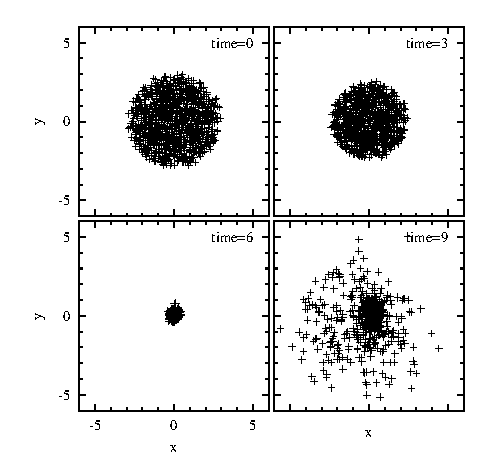
\includegraphics[width=10cm,bb=0 0 220 220]{fig/nbody.eps}
  \end{center}
  \caption{}
  \label{fig:nbody}
\end{figure}

\subsubsubsection{Phantom-GRAPEの利用}

以下では、相互作用計算にPhantom-GRAPEを使う場合について、記述する。この
場合、ユーザーはまずはPhantom-GRAPEのコンパイルを行わなければならない。
今回使うPhantom-GRAPEのソースコードは、
\texttt{fdps/FDPS-master/src/phantom\_grape\_x86/G5/newton/libpg5/} 以
下に存在するので、そこまで移動し、コンパイルを行う。以下は、現在
\texttt{sample/nbody/}に居る場合の例である。
\begin{screen}
\begin{verbatim}
$ cd ../../src/phantom_grape_x86/G5/newton/libpg5/
$ make
\end{verbatim}
\end{screen}

コンパイルが成功したら、元のディレクトリに戻る。次に、
\texttt{Makefile}の修正を行う。\texttt{Makefile}の11行目に
Phantom-GRAPEを使用するか否かを決定しているスイッチが存在している。この
スイッチはデフォルトではコメントアウトされて\texttt{no}になっているいる
ため、以下のようにしてコメントアウトを解除する。
\begin{screen}
\begin{verbatim}
use_phantom_grape_x86 = yes
\end{verbatim}
\end{screen}

無事にコンパイルが通れば、以降の実行・解析の手順は同様である。実行直後
に次のような表示がされれば、正しく実行ができている。
\begin{screen}
\begin{verbatim}
******** FDPS has successfully begun. ********
./result/t-de.dat
Number of processes: 1
Number of threads per process: 1
rsqrt: MSE = 1.158186e-04,  Bias = 8.375360e-08
(以下省略)
\end{verbatim}
\end{screen}

\subsubsubsection{OpenMP/MPIの利用}

OpenMPやMPIを利用する場合について以下に記述する。

以降では、計算の実行の際にはジョブの投入を行うことにする。今回は以下の
様なコマンドでジョブの投入を行う。これはOpenMP実行の際の例である。
\begin{screen}
\begin{verbatim}
$ sbatch runOMP.sh
\end{verbatim}
\end{screen}
正しくジョブが投入されている場合、\texttt{squeue}コマンドを実行すると、例えば以
下のようにログが出力される。
\begin{screen}
\begin{verbatim}
 JOBID PARTITION     NAME     USER ST       TIME  NODES NODELIST(REASON)
200402     d006h    nbody uleo0016 PD       0:00      1 (None)
\end{verbatim}
\end{screen}
ジョブのキャンセルは以下のコマンドで実行できる。
\begin{screen}
\begin{verbatim}
$ scancel JOBID
\end{verbatim}
\end{screen}
JOBIDは上の\texttt{squeue}コマンドで表示されたJOBIDの番号である(上で言えば、
200402)。
正しくジョブが終了すると、ファイル\texttt{stdout.log}の最後にログが出力される。


\begin{itemize}
\item OpenMPのみ使用の場合
  \begin{itemize}
  \item \texttt{Makefile}の編集
    \begin{itemize}
    \item マクロ\texttt{CC}にOpenMP対応のC++コンパイラを代入する。
          今回の実習の環境では変更する必要は無い。
    \item ``\texttt{CFLAGS += -DPARTICLE\_SIMULATOR\_THREAD\_PARALLEL -fopenmp}''の
      行のコメントアウトを外す
    \end{itemize}
  \item \texttt{make}コマンドを実行する。
  \item \texttt{sbatch runOMP.sh}と打って実行する。正しく実行された場合、stdout.logに以下のように表示されるはずである。
\begin{screen}
\begin{verbatim}
******** FDPS has successfully begun. ********
./result/t-de.dat
Number of processes: 1
Number of threads per process: 4
rsqrt: MSE = 1.158186e-04,  Bias = 8.375360e-08
(以下省略)
\end{verbatim}
\end{screen}
       見て分かる通り、\texttt{Number of threads per process: 4}となっている。
       これで、4スレッドでの並列計算が行われている事が確認できた。
  \end{itemize}

\item OpenMPとMPIの同時使用の場合
  \begin{itemize}
  \item \texttt{Makefile}の編集
    \begin{itemize}
    \item マクロ\texttt{CC}にMPI対応のC++コンパイラを代入する。
          今回の実習の環境では\texttt{mpic++}にする。
    \item ``\texttt{CFLAGS += -DPARTICLE\_SIMULATOR\_THREAD\_PARALLEL -fopenmp}''の
      行のコメントアウトを外す(インテルコンパイラの場合は\texttt{-fopenmp}を外す)
    \item ``\texttt{CFLAGS += -DPARTICLE\_SIMULATOR\_MPI\_PARALLEL}''の行のコメント
      アウトを外す
    \end{itemize}
  \item \texttt{make}コマンドを実行する。
  \item \texttt{sbatch runMPI.sh}と打って実行する。正しく実行された場合、stdout.log以下のように表示されるはずである。
\begin{screen}
\begin{verbatim}
(省略)
******** FDPS has successfully begun. ********
./result/t-de.dat
./result/t-de.dat
Number of processes: 2
Number of threads per process: 4
rsqrt: MSE = 1.158186e-04,  Bias = 8.375360e-08
rsqrt: MSE = 1.158186e-04,  Bias = 8.375360e-08
(以下省略)
\end{verbatim}
\end{screen}
       見て分かる通り、\texttt{Number of processes: 2}となっている。
       これで、2プロセス4スレッドでの並列計算が行われている事が確認できた。
  \end{itemize}

\end{itemize}

\subsubsection{SPHシミュレーションコード}

\subsubsubsection{概要}

ここでは、SPHシミュレーションコードを動かす。用意されているコードは、断
熱スフィアコラプスの計算を行う。この節でまず行うことは、シリアルコード
のコンパイルと実行、出て来た結果の解析である。最後にOpenMPやMPI を利用
して、さらにコードを高速化する。

\subsubsubsection{シリアルコード}

以下の手順で本コードを使用できる。
\begin{itemize}
\item ディレクトリ\texttt{fdps/FDPS-master/sample/nbodysph}に移動
\item \texttt{make}を実行
\item ジョブの投入
\item 結果の解析
\item OpenMP/MPIの利用(オプション)
\end{itemize}

\subsubsubsubsection{ディレクトリ移動}

ディレクトリ\texttt{fdps/FDPS-master/sample/nbodysph}に移動に移動する。

\subsubsubsubsection{makeの実行}

\texttt{make}コマンドを実行する。

\subsubsubsubsection{計算の実行}
まずは、インタラクティブ実行で計算を実行する。
これは、生成された実行ファイルの名前をそのまま実行すればよい。
\begin{screen}
\begin{verbatim}
$ ./sph.out
\end{verbatim}
\end{screen}

正しくジョブが終了すると、標準入出力の最後には以下のようなログが出力されるはずである。
\begin{screen}
\begin{verbatim}
(省略)
//================================
time = 7.6861124696015781e-01, dt = 3.5727841270539857e-03
step = 88
//================================
9.9999999999997635e-01
6.6872858041836647e-01
9.7700092080239072e-04
9.7700092080317243e-04
9.7700092080318761e-04
******** FDPS has successfully finished. ********
\end{verbatim}
\end{screen}

\subsubsubsubsection{結果の解析}

ディレクトリ\texttt{result}にファイルが出力されている。ファイル名は"00**.dat"(*
には数字が入る)となっている。ファイル名は時刻を表す。出力ファイルフォー
マットは1列目から順に粒子のID、粒子の質量、位置の$x$, $y$, $z$ 座標、粒子の
$x$, $y$, $z$軸方向の速度、密度、内部エネルギー、圧力である。

これは3次元のEvrard sphereである。以下のコマンドを実行すれば、横軸に
$r$、縦軸に密度のlogscaleでの図が作成される。

\begin{screen}
\begin{verbatim}
$ gnuplot
$ set logscale
$ plot "result/0040.dat" using (sqrt($3**2 + $4**2 + $5**2)):9
\end{verbatim}
\end{screen}
正しい答が得られれば、図\ref{fig:sph}のような図を描ける。

\begin{figure}
  \begin{center}
%    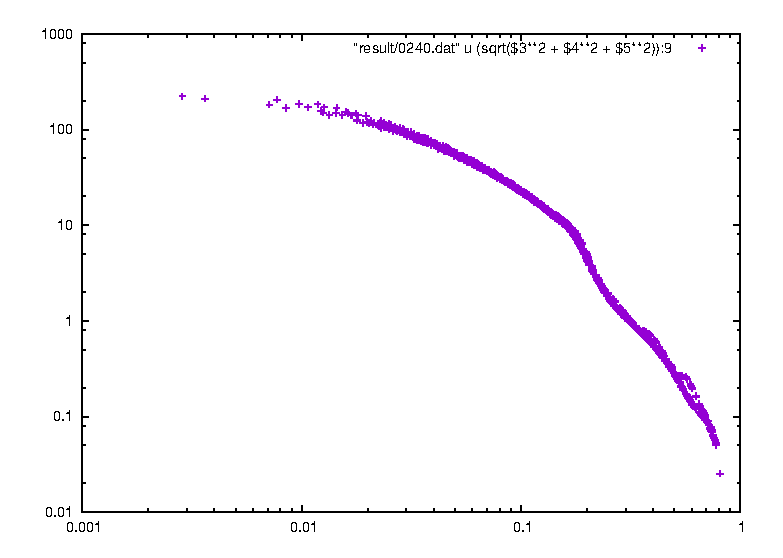
\includegraphics[]{fig/sph.eps}
    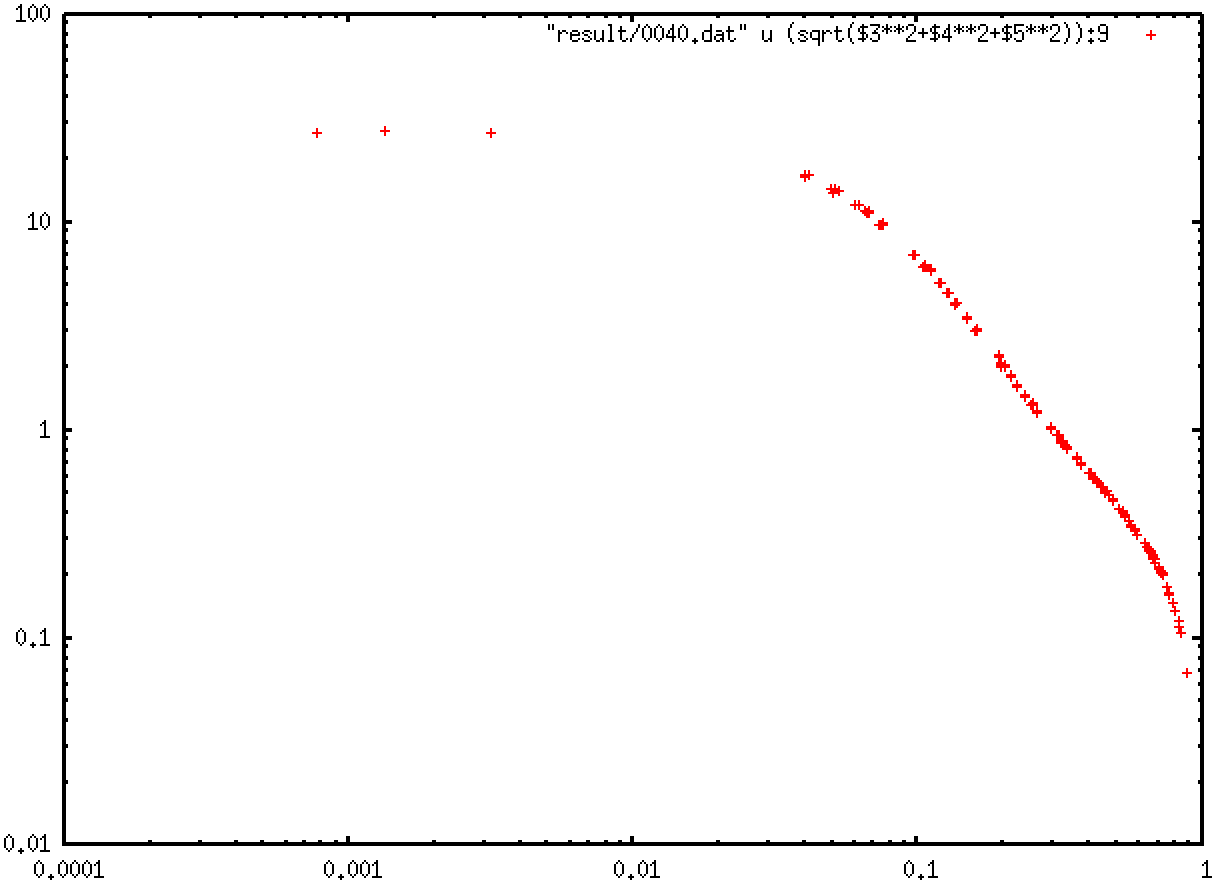
\includegraphics[width=10cm,bb=0 0 608 444]{fig/sph.png}
  \end{center}
  \caption{}
  \label{fig:sph}
\end{figure}

\subsubsubsection{OpenMP/MPIの利用}

OpenMPやMPIを利用する場合を以下に示す。
\begin{itemize}
\item OpenMPのみ使用の場合
  \begin{itemize}
  \item \texttt{Makefile}の編集
    \begin{itemize}
    \item マクロ\texttt{CC}にOpenMP対応のC++コンパイラを代入する
    \item ``\texttt{CFLAGS += -DPARTICLE\_SIMULATOR\_THREAD\_PARALLEL -fopenmp}''の
      行のコメントアウトを外す
    \end{itemize}
  \item \texttt{make}コマンドを実行する。
  \item \texttt{sbatch runOMP.sh}と打って実行する。正しく実行された場合、stdout.log以下のように表示されるはずである。
\begin{screen}
\begin{verbatim}
******** FDPS has successfully begun. ********
//==================================\\
||                                  ||
|| ::::::: ::::::. ::::::. .::::::. ||
|| ::      ::    : ::    : ::       ||
|| ::::::  ::    : ::::::'  `:::::. ||
|| ::      ::::::' ::      `......' ||
||     Framework for Developing     ||
||        Particle Simulator        ||
\\==================================//
//=====================================
This is a sample program of Smoothed Particle Hydrodynamics on FDPS!
# of proc is   1
# of thread is 4
//=====================================
\end{verbatim}
\end{screen}
  \end{itemize}

\item OpenMPとMPIの同時使用の場合
  \begin{itemize}
  \item \texttt{Makefile}の編集
    \begin{itemize}
    \item マクロ\texttt{CC}にMPI対応のC++コンパイラを代入する
    \item ``\texttt{CFLAGS += -DPARTICLE\_SIMULATOR\_THREAD\_PARALLEL -fopenmp}''の
      行のコメントアウトを外す(インテルコンパイラの場合は\texttt{-fopenmp}を外す)
    \item ``\texttt{CFLAGS += -DPARTICLE\_SIMULATOR\_MPI\_PARALLEL}''の行のコメント
      アウトを外す
    \end{itemize}
  \item \texttt{make}コマンドを実行する。
  \item \texttt{sbatch runMPI.sh}と打って実行する。正しく実行された場合、stdout.log以下のように表示されるはずである。
\begin{screen}
\begin{verbatim}
******** FDPS has successfully begun. ********
//==================================\\
||                                  ||
|| ::::::: ::::::. ::::::. .::::::. ||
|| ::      ::    : ::    : ::       ||
|| ::::::  ::    : ::::::'  `:::::. ||
|| ::      ::::::' ::      `......' ||
||     Framework for Developing     ||
||        Particle Simulator        ||
\\==================================//
//=====================================
This is a sample program of Smoothed Particle Hydrodynamics on FDPS!
# of proc is   2
# of thread is 4
//=====================================
\end{verbatim}
\end{screen}
  \end{itemize}
\end{itemize}

\end{document}
